% This is a sample file for the Undergraduate Faculty Program at
% PCMI, containing one lecture 
%
%
% The sample file illustrates the use of epsf.tex to include postscript 
% graphics, as well as various "AmS-LaTeX" constructions from the amsmath
% package (which is automatically loaded by the pcms-l document class).
% To run this file you need the files 
%
%        pcms-l.cls and pcmslmod.tex
%


\documentclass[lecture,12pt,]{pcms-l}
\input pcmslmod.tex  % v.1.2
%\input epsf.tex
\usepackage[framed,numbered,autolinebreaks,useliterate]{mcode}
\usepackage{graphicx}
\usepackage{subcaption}
\usepackage[toc,page]{appendix}
%\usepackage{natbib}
%\usepackage{amssymb} % this command would have loaded all the extra symbols,



% authors should not define these, they will be defined by the volume editors
%\def\currentvolume{3}
%\def\currentyear{1993}


% EQUATION NUMBERING AND THEOREM SETUP

\numberwithin{section}{chapter}
\numberwithin{equation}{chapter}

\theoremstyle{plain}
\newtheorem{theorem}[equation]{Theorem}
\newtheorem{lemma}[equation]{Lemma}

\theoremstyle{definition}
\newtheorem{example}{Example}[section]

\theoremstyle{definition}
\newtheorem{definition}[equation]{Definition}

\newtheorem{exercise}{Exercise}
\newtheorem{problem}{Problem}
\newtheorem*{remark}{Remark}

% Set enumerate to use letters, not numbers for problem parts.

\renewcommand{\theenumi}{\alph{enumi}}
\renewcommand{\labelenumi}{(\theenumi)}

% AUTHOR-DEFINED MACROS:

\newcommand{\cA}{\mathcal{A}}
\newcommand{\cB}{\mathcal{B}}
\newcommand{\C}{\mathbb{C}}
\newcommand{\cC}{\mathcal{C}}
\newcommand{\cD}{\mathcal{D}}

\begin{document}

\mainmatter
\setcounter{page}{1}

%\LogoOn

\lectureseries[Bayesian Analysis]{Decision Theory and Bayesian Analysis}


\auth[Dr. Vilda Purutcuoglu]{Dr. Vilda Purutcuoglu}
\address{Tubitak Space Technologies Research Institute, Ankara, 06800, Turkey}

\footnote{Edited by Anil A. Aksu based on lecture notes of STAT 565 course by Dr. Vilda Purutcuoglu }
%\email{ajb@hmc.edu}



% the following hack starts the lecture numbering at 1
\setcounter{lecture}{0}
\setcounter{chapter}{0}
\tableofcontents
%\listoffigures

\lecture{Bayesian Paradigm}

%\section{Outline of Lecture}
%\begin{itemize}
%\item{What is a Partial Differential Equation?}
%\item{Classifying PDE's: Order, Linear vs. Nonlinear}
%\item{Homogeneous PDE's and Superposition}
%\item{The Transport Equation} 
%\end{itemize}


\section{Bayes theorem for distributions}

If $A$ and $B$ are two events,
\begin{equation}
P(A\mid B)=\frac{P(A)P(B\mid A)}{P(B)}.
\end{equation}
This is just a direct consequence of the multiplication law of probabilities that says we can express $P(A\mid B)$ as either $P(A)P(B\mid A)$ or $P(B)P(A\mid B)$. For discrete distributions, if $Z,Y$ are discrete random variables
\begin{equation}
\label{eq:1}
P(Z=z\mid Y = y)=\frac{P(Z =z)P(Y = y\mid Z =z)}{P(Y = y)}.
\end{equation}
\begin{itemize}
\item How many distributions do we deal with here?
\end{itemize}
We can express the denominator in terms of the distribution in the numerator\cite{Allen}.
\begin{equation}
P(Y = y)=\sum_z P(Y = y, Z =z)=\sum_z P(Z= z)P(Y = y\mid Z =z).
\end{equation}
\begin{itemize}
\item This is sometimes called the law of total probability 
\end{itemize}
In this context, it is just an expression of the fact that as $z$ ranges over the possible values of $Z$
, the probabilities on the left hand-side of equation \ref{eq:1} make up the distribution of $Z$ given $Y=y$, and so they must add up to one. The extension to continuous distribution is easy. If $Z,Y$ are continuous random variable,
\begin{equation}
f(Z\mid Y)=\frac{f(Z)f(Y\mid Z)}{f(Y)}.
\end{equation}
where the denominator is now expressed as an integral:
\begin{equation}
f(Y)=\int f(Z)f(Y\mid Z)\mathrm{d}Z.
\end{equation}
\begin{equation}
f=
\left\{\begin{matrix}
continous \quad name ?\\ 
discrete \quad name ?
\end{matrix}\right.
\end{equation}


\vfill
%\begin{center}
%{\it (Room for notes)}
%\end{center}
\eject

\section{How Bayesian Statistics Uses Bayes Theorem}
\begin{theorem}[Bayes' theorem]
\label{Bayes}
\[P(A\mid B)=\frac{P(A)P(B\mid A)}{P(B)}\]
$P(B)$=if we are interested in the event $B$, $P(B)$ is the initial or prior probability of the occurence of event $B$. Then we observe event $A$ 
\\
$P(B\mid A)=$ How likely $B$ is when $A$ is known to have occurred is the posterior probability $P(B\mid A)$. 
\end{theorem}
Bayes' theorem can be understood as a formula for updating from prior to posterior probability, the updating consists of multiplying by the ratio $P(B\mid A)/P(A)$. It describes how a probability changes as we learn new information. Observing the occurrence of $A$ will increase the probability of $B$ if $P(B\mid A)>P(A)$.
From the law of total probability,
\begin{equation}
P(A)=P(A\mid B)P(B)+P(A\mid B^c)P(B^c).
\end{equation}
where $P(B^c)=1-P(B)$.
\begin{lemma}
\[P(A\mid B)-P(A)=\frac{P(A)-P(A\mid B^c)P(B^c)}{1-P(B^c)}-P(A)\]
\end{lemma}
 
\begin{proof}
\[P(A\mid B)-P(A)=\frac{P(A)-P(A\mid B^c)P(B^c)-P(A)+P(A)P(B^c)}{P(B)}\]
\[P(A\mid B)-P(A)=\frac{P(B^c)(P(A)-P(A\mid B^c))}{P(B)}\]
\[P(A\mid B)-P(A)=P(B^c)(\frac{P(B)P(A\mid B)+P(B^c)P(A\mid B^c)}{P(B)}-\frac{P(A\mid B^c)}{P(B)})\]
\[P(A\mid B)-P(A)=P(B^c)(P(A\mid B)-\frac{P(A\mid B^c)(1-P(B^c))}{P(B)})\]
\[P(A\mid B)-P(A)=P(B^c)(P(A\mid B)-P(A\mid B^c))\]
\end{proof}
\subsection{Generalization of the Bayes' Theorem}
Let $B_1,...,B_n$ be a set of mutually exclusive events. Then
\begin{equation}
P(B_r\mid A)=\frac{P(B_r)P(A\mid B_r)}{P(A)}=\frac{P(B_r)P(A\mid B_r)}{\sum_{i=1}^n P(B_r)P(A\mid B_r)}.
\end{equation}
\begin{itemize}
\item Assuming that $P(B_r)>0$,$P(A\mid B)>P(A)$ if and only if $P(A\mid B)>P(A\mid B^c)$.
\item In Bayesian inference we use Bayes' theorem in a particular way.
\item $Z$ is the parameter (vector) $\theta$.
\item $Y$ is the data (vector) $X$.
\end{itemize}
So we have 
\begin{equation}
f(\theta\mid X)=\frac{f(\theta)f(X\mid \theta)}{f(X)}
\end{equation}
\begin{equation}
f(X)=\int f(\theta)f(X\mid \theta)\mathrm{d}\theta.
\end{equation}
\begin{equation}
f(\theta)=prior.
\end{equation}
\begin{equation}
f(\theta\mid X)=posterior.
\end{equation}
\begin{equation}
f(X\mid \theta)=likelihood.
\end{equation}
\subsection{Interpreting our sense} 
How do we interpret the things we see, hear, feel, taste or smell?
\begin{example}
I hear a song on the radio I identify the singer as Robbie Williams. Why do I think it's Robbie Williams?. Because he sounds like that. Formally, $P($ What I hear Robbie Williams $)>>P($What I hear someone else $)$
\end{example}
\begin{example}
I look out of the window and see what appears to be a tree. It has a big, dark coloured part sticking up out of the ground that branches into thinner sticks and on the ends of these are small green things. Clearly, $P(view \mid  tree)$ is high and $P(view \mid car)$ or $P(view \mid Robbie \quad Williams)$ are very small. But $P(view \mid carboard \quad cutout \quad cunningly \quad painted \quad to \quad look \quad like \quad a \quad tree)$ is also very high. Maybe even higher than $P(view \mid  tree)$ in the sense that what I see looks almost like a tree.
\\
Does this mean I should now believe that I am seeing a cardboard cut-out cunningly painted to look like a tree? No because it is much less likely to begin with than a red tree.
\end{example}
In statistical terms, consider some data $X$ and some unknown parameter $\theta$. The first step in any statistical analysis is to build a model that links the data to unknown parameters and the main function of this model is to allow us to state the probability of observing any data given any specified values of the parameters. That is the model defines $f(x\mid \theta)$. 
\\
When we think of $f(x\mid \theta)$ as a function of $\theta$ for fixed observed data $X$, we call it likelihood function and it by $L(\theta,X)$.
\begin{itemize}
\item So how can we combine this with our example?
\end{itemize}
This perspective underlies the differences between the two main theories of statistical inference.
\begin{itemize}
\item Frequentist inference essentially uses only the likelihood, it does not recognize $f(\theta)$.
\item Bayesian inference uses both likelihood and $f(\theta)$.
\end{itemize}
The principal distinguishing feature of Bayesian inference as opposed to frequentist inference is its use of $f(\theta)$.

\section{Prior to Posterior}
We refer to $f(\theta)$ as the \underline{prior distribution} of $\theta$. It represents knowledge about $\theta$ prior to observing the data $X$. We refer to $f(\theta \mid X)$ as the \underline{posterior distribution} of $\theta$ and it represents knowledge about $\theta$ after observing $X$. 
\begin{itemize}
\item So we have two sources of information about $\theta$.
\item Here $f(x)$ does not depend on $\theta$. Thus $\int f(\theta \mid x) \mathrm{d} \theta=1$. Since $f(x)$ is a constant within the integral, we can take it outside to get $1=f^{-1}(x)\int f(\theta) f(x \mid \theta) \mathrm{d}\theta$.
\item $f(\theta \mid x)= \propto f(\theta) f(x \mid \theta)\propto f(\theta) L(\theta ; x)$ (the posterior is proportional to the prior times the likelihood).
\item The constant that we require to scale the right hand side to integrate to $1$ is usually called the normalizing constant. If we haven't dropped any constants form $f(\theta)$ or $f(x \mid \theta)$, then the normalising constant is just $f^{-1}(x)$, otherwise it also restores any dropped constants. 
\end{itemize}
\section{Triplot}
If for any value of $\theta$, we have either $f(\theta)=0$ or $f(x\mid \theta)=0$, then we will also have $f(\theta \mid x)=0$. This is called the property of zero preservation. So if either:
\begin{itemize}
\item the prior information says that this $\theta$ value is impossible
\item the data say that this value of $\theta$ is impossible because if it were the true value, then the observed data would have been impossible, then the posterior distribution confirms that this value of $\theta$ is impossible.
\end{itemize}

\begin{definition}{Crowwell's Rule:}
If either information source completely rules out a specific $\theta$, then the posterior must rule it out too. This means that we should be very careful about giving zero probability to something unless it is genuinely impossible. Once something has zero probability then no amount of further evidence can cause it to have a non-zero posterior probability.
\end{definition}

\begin{itemize}
\item More generally, $f(\theta \mid x)$ will be low if either $f(\theta)$ is very small.  We will tend to find that $f(x \mid \theta)$ is large when both $f(\theta)$ and $f(x \mid \theta)$ are relatively large, so that this $\theta$ value is given support by \underline{both} information sources.
\end{itemize}
When $\theta$ is a scalar parameter, a useful diagram is the \underline{triplot}, which shows the prior, likelihood and posterior on the same graph. An example is in Figure \ref{fig:Triplot}.\footnote{All plots are generated in R, relevant codes are provided in Appendix R Codes }
\begin{figure}
\centering
 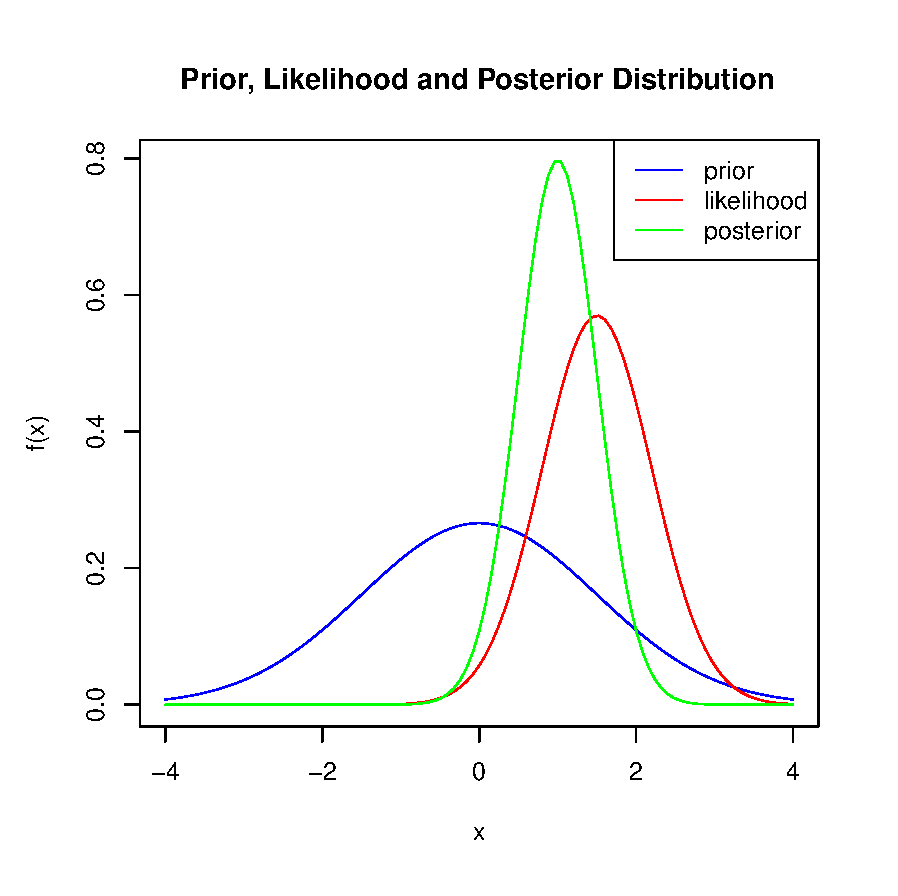
\includegraphics[scale=0.7]{triplot}% Images in 100% size
  \caption{Triplot of prior, likelihood and posterior. }
\label{fig:Triplot}
\end{figure} 
\\
\\
A strong information source in the triplot is indicated by a curve that is narrow (and therefore, because it integrates to one, also has a high peak). A narrow curves concentrates on a small range of $\theta$ values, and thereby "rules out" all values of $\theta$ outside that range.

\vfill
\eject
\begin{itemize}
\item Over the range $\theta<-1$, the likelihood: low
\item Over the range $\theta>3$,the likelihood: low
\item Values of $\theta$ between $-1$ and $3$, the likelihood: high
\item The maximum value of the posterior at: $1$
\item The Maximum likelihood estimation (MLE) of $\theta$ is $\approx 2$
\end{itemize}
\subsection{Normal Mean}
For example, suppose that $X_1, X_2,...,X_n$ are iid $ \mathcal{N}(\mu,\,\sigma^{2})$ and $\sigma^2$ is known. Then the likelihood is :
\begin{equation}
\begin{split}
f(x \mid \mu)= \prod_{i=1}^{n}f(x_i \mid \mu)=\prod_{i=1}^{n}\frac{1}{\sqrt{2\pi}\sigma}\exp\left (  -\frac{1}{2\sigma^2}(x_i -\mu)^2 \right )
\\
\propto \exp\left (  -\frac{1}{2\sigma^2}(x_i -\mu)^2 \right ).
\end{split}
\end{equation}
As,
\begin{equation}
\begin{split}
\sum (x_i-\bar{x}+\bar{x}-\mu)^2=\sum (x_i-\bar{x})^2+n(\bar{x}-\mu)^2+2(\bar{x}-\mu)\sum(x_i-\bar{x})
\\
=\sum (x_i-\bar{x})^2+n(\bar{x}-\mu)^2
\\
\propto \exp\left (  -\frac{1}{2\sigma^2}n(\bar{x} -\mu)^2 \right ).
\end{split}
\end{equation}
Note that $2(\bar{x}-\mu)\sum(x_i-\bar{x})=0$ as $\sum(x_i-\bar{x})=0$. Suppose the prior distribution for $\mu$ is normal:
\begin{equation}
\mu \sim \mathcal{N}(m,v).
\end{equation}
Then applying Bayes' theorem we have:
\begin{equation}
\begin{split}
f(\mu \mid x) \propto \underbrace{\exp\left (  -\frac{1}{2\sigma^2}n(\bar{x} -\mu)^2 \right )}_{f(x \mid \mu)} \underbrace{\exp\left (  -\frac{1}{2 v}n(\mu-m)^2 \right )}_{f(\mu)}
\\
=\exp\left (  -\frac{\theta}{2} \right ).
\end{split}
\end{equation}
Note that
\begin{equation}
\theta=n \sigma^{-2}(\bar{x}-\mu)+v^{-1}(\mu-m)^2=(v^*)^{-1}(\mu-m^*)^2+R
\end{equation}
and 
\begin{equation}
v^*=(n\sigma^{-2}+v^{-1})^{-1}
\end{equation}
\begin{equation}
m^*=(n\sigma^{-2}+v^{-1})^{-1}(n \sigma^{-2}\bar{x}+v^{-1}m)=a \bar{x}+(1-a)m 
\end{equation}
where $a=n \sigma^-2/(n \sigma^{-2}+v^{-1})$
\begin{equation}
R=(n^{-1}\sigma^2+v)(\bar{x}-m)^2
\end{equation}
Therefore,
\begin{equation}
f(\mu \mid x) \propto \exp\left (  -\frac{1}{2 v}n(\mu-m)^2 \right )
\end{equation}
and we have shown that the posterior distribution is normal too: $\mu \mid x \sim \mathcal{N}(m^*,\,v^*)$
\begin{itemize}
\item $m^*=$ weighted average of the mean $m$ and the usual frequentist data-only estimate $\bar{x}$. 
\\
The weights $\propto$:
\item Bayes' theorem typically works in this way. We \underline{usually} find that posterior estimates are compromises between prior estimates and data based estimates and tend to be closer whichever information source is stronger. And we \underline{usually} find that the posterior variance is smaller than the prior variance.
\end{itemize}
\subsection{Weak Prior Information}
It is the case where the prior information is much weaker that the data. This will occur, for instance, if we do not have strong information about $Q$ before seeing the  data, and if there are lots of data. Then in triplot, the prior distribution will be much broader and flatter that the likelihood. \underline{So the posterior is approximately proportional to the likelihood.}
\begin{example}
In the normal mean analysis, we get weak prior information by letting the prior precision of $v^{-1}$ become small. Then $m^* \rightarrow \bar{x}$ and $v^* \rightarrow \sigma^2/n$ so that the posterior distribution of $\mu$ corresponds very closely with standard frequentist theory.
\end{example}



\vfill
\eject




\lecture{Some Common Probability Distributions}
\underline{\bf{Binomial}} on $Y \in \left \{0,1,...,n  \right \}$ with parameters $n \in \left \{1,2,3,... \right \}$ and $p \in (0,1)$ is denoted by $Bi(n,p)$ and 
\begin{equation}
f(y \mid n, p)=\binom{n}{y}p^y (1-p)^{n-y}
\end{equation}
for $y=0,1,...,n$. The mean is given as:
\begin{equation}
E(y)=np.
\end{equation}
Also the variance is given as:
\begin{equation}
v(y)=np(1-p).
\end{equation}
\underline{\bf{Beta}} on  $Y \in \left \{0,1 \right \}$ with parameters $a,b>0$ is denoted by $Beta(p,q)$ and the density function is:
\begin{equation}
f(y \mid p,q)= \frac{\Gamma(p+q)}{\Gamma(p)\Gamma(q)}y^{p-1}(1-y)^{q-1}
\end{equation}
for $y \in (0,1)$. The mean is given as:
\begin{equation}
E(y)=\frac{p}{p+q},
\end{equation}
Also the variance is given as:
\begin{equation}
v(y)=\frac{pq}{(p+q)^2(p+q+1)}.
\end{equation}
$B(p,q)=\int_{0}^1 y^{p-1}(1-y)^{q-1}\mathrm{d}y$ is the beta function and defined to be the normalizing constant for this density.
\begin{itemize}
\item In beta distribution, $p$ and $q$ change the shape of the distribution. Discuss!
\end{itemize}
\underline{\bf{Uniform distribution}} on $Y \in \left \{l,r \right \}$ where $-\infty<l<r<\infty$ is denoted by uniform $(l,r)$ and its pdf is:
\begin{equation}
f(y\mid l,r)=\frac{1}{r-l}
\end{equation}
for $y \in \left \{l,r \right \}$. The mean is given as:
\begin{equation}
E(y)=\frac{l+r}{2},
\end{equation}
Also the variance is given as:
\begin{equation}
v(y)=\frac{(r-l)^2}{12}.
\end{equation}
\underline{\bf{Poisson distribution}} on $Y \in \left \{0,1,2,..., \right \}$ with parameter $\theta>0$ is denoted by $Poisson(\theta)$ and its pdf is:
\begin{equation}
f(y \mid \theta)=\frac{\exp(-\theta)\theta^y}{y!}
\end{equation}
for $y=0,1,2,..$. The mean and the variance are given as\cite{Ross}:
\begin{equation}
E(y)=v(y)=\theta.
\end{equation}
\underline{\bf{Gamma distribution}} on $Y > 0$ with shape parameter $\alpha>0$ and rate parameter $\lambda>0$ is denoted by $Gamma(\alpha,\lambda)$ and the corresponding density is:
\begin{equation}
f(y \mid \alpha, \lambda)=\frac{\lambda^{\alpha}}{\Gamma(\alpha)} y^{\alpha-1} \exp(-\lambda y)
\end{equation}
for $y>0$. The mean is given as:
\begin{equation}
E(y)=\frac{\alpha}{\lambda},
\end{equation}
Also the variance is given as:
\begin{equation}
v(y)=\frac{\alpha}{\lambda^2}.
\end{equation}
Note that 
\begin{equation}
\exp(\lambda)=Gamma(1,\lambda).
\end{equation}
\underline{\bf{Univariate normal distribution}} on $Y \in \mathbb{R}$ with $\mu \in \mathbb{R}$ and variance $\sigma^2>0$ is denoted by $\mathcal{N}(\mu,\sigma^2)$ and its pdf is:
\begin{equation}
f(y \mid \mu, \sigma^2)=\frac{1}{\sigma} \left (  \frac{1}{2 \pi}\right )^{1/2} \exp \left \{ -\frac{1}{2 \sigma^2}(y -\mu)^2  \right \}.
\end{equation}
 The mean is given as:
\begin{equation}
E(y)=\mu,
\end{equation}
Also the variance is given as:
\begin{equation}
v(y)=\sigma^2.
\end{equation}
\underline{\bf{K-variate normal distribution}} on $Y \in \mathbb{R}^k$ with vector $\mathbf{b} \in \mathbb{R}^k$ and positive definite symmetric (PDS) covariance matrix $\mathbf{C}$ is denoted by $\mathcal{N}_k(\mathbf{b},\mathbf{C})$ and the corresponding density function is:
\begin{equation}
f(y \mid \mathbf{b},\mathbf{C})=\frac{1}{\underbrace{\left | \mathbf{C} \right |^{1/2}}_{determinant}}\frac{1}{(2 \pi)^{k/2}}\exp \left \{ -\frac{1}{2 \sigma^2}(y -\mathbf{b})^T \mathbf{C}^{-1}(y-\mathbf{b}) \right \}.
\end{equation}
 The mean is given as:
\begin{equation}
E(y)=\mathbf{b},
\end{equation}
And the covariance matrix is given as:
\begin{equation}
Cov(y)=\mathbf{C}.
\end{equation}
\section{Posterior}
Not only the beta distributions are the simplest and the most convenient distributions for a random variable confined to $[0,1]$, they also work very nicely as prior distribution for a binomial observation. If $\theta \sim Be(p,q)$ then
\begin{equation}
f(x \mid \theta)=\binom{n}{x}\theta^x (1-\theta)^{n-x}.
\end{equation}
for $x=1,2,...,n$.
\begin{equation}
f(\theta)=\frac{1}{Be(p,q)}\theta^{p-1}(1-\theta)^{q-1}
\end{equation}
where $0\leq \theta \leq 1$ and $p,q>0$.
\begin{equation}
\begin{split}
f(x)=\int f(\theta)f(x \mid \theta)\mathrm{d}\theta=\binom{n}{r}\frac{1}{Be(p,q)}\int_{0}^{1}\theta^{p+x-1}(1-\theta)^{q+n-x-1}\mathrm{d}\theta
\\
=\binom{n}{r}\frac{Be(p+x,q+n-x)}{Be(p,q)}.
\end{split}
\end{equation}
From
\begin{equation}
f(\theta \mid x)=\frac{f(\theta)f(x \mid \theta)}{f(x)}.
\end{equation}
\begin{equation}
\begin{split}
f(\theta \mid x)=\frac{\theta^{p+x-1}(1-\theta)^{q+n-x-1}}{Be(p+x,q+n-x)}
\propto \underbrace{\theta^{p-1}(1-\theta)^{q-1}}_{Beta \quad part} \underbrace{\theta^{x}(1-\theta)^{n-x}}_{Binomial \quad part}. 
\end{split}
\end{equation}
So $(\theta \mid x)\propto Beta(p+x,q+n-x)$. The posterior mean is:
\begin{equation}
\begin{split}
E(\theta \mid x)= \frac{p+x}{p+q+n}=\frac{p+q}{p+q+n}E(\theta)+\frac{n}{p+q+n}\hat{\theta}
\end{split}
\end{equation}
where $\hat{\theta}=x/n$. The posterior variance is:
\begin{equation}
\begin{split}
v(\theta \mid x)=\frac{(p+x)(q+n-x)}{(p+q+n)^2 (p+q+n+1)}
\\
=\frac{E(\theta)(1-E(\theta \mid x))}{ p+q+n+1}
\end{split}
\end{equation}
But,
\begin{equation}
v(\theta)=\frac{E(\theta)(1-\theta)}{p+q+1}
\end{equation}
So the posterior has higher relative precision that the prior.
\\
\underline{\bf{SPECIAL NOTE:}}
\\
The classical theory of estimation regards an estimator as good if it is unbiased and has small variance, or more generally if its mean-square-error is small. The MSE is an average squared error where the error is the difference between $\theta$, i.e. $y$ in previous notation , and the estimate $t$. In accordance with classical theory, the average is taken with respect to the sampling distribution of the estimator.
\\
In Bayesian inferenc, $\theta$ is a random variable and it is therefore appropriate to average the squared error with respect to the posterior distribution of $\theta$. Consider
\begin{equation}
\begin{split}
E\left \{ (t -\theta)^2 \mid x \right \}=E(t^2 \mid x)- E(2 t \theta \mid x)+ E(\theta^2 \mid x)
\\
= t^2 - E(2 t \theta \mid x)+ E(\theta^2 \mid x)
\\
=\left \{ t - E(\theta \mid x)\right \}^2+v(\theta \mid x).
\end{split}
\end{equation} 
Therefore the estimate $t$ which minimizes posterior expected square error is $t=E(\theta \mid x)$, the posterior mean. The posterior mean can therefore be seen as an estimate of $\theta$ which is the best in the sense of minimizing expected squared error. This is distinct from, but clearly related to, its more natural role as a useful summary of location of the posterior distribution. 
\section{Weak Prior}
If we reduce the prior relative precision to zero by setting $p=q=0$, we get $\theta \mid x \sim Be(x,n-x)$. Then $E(\theta \mid x)=\hat{\theta}$ and $v(\theta \mid x)=\hat{\theta}(1-\hat{\theta})/(n+1)$ results which nicely parallel standard frequentist theory.
\begin{itemize}
\item Notice that we are not really allowed to let either parameter of the beta distribution be zero. However, by making $p$ and $q$ extremely small, we get as close to these results as we like. We can think of $p=q=0$ as a defining limiting (if strictly improper) case of weak prior information.
\end{itemize}

\begin{example}
A doctor proposes a new treatment protocol for a certain kind of cancer. With current methods about $40 \%$ of patients with this cancer survive six months after diagnosis. After one year of using the new protocol, $15$ patients with diagnosis, of whom $6$ survived. After two years a further $55$ patients have been followed to teh six months mark, of whom $28$ survived. So in total we have $34$ patients surviving out of $70$.
\\
Let $\theta$ be the true success rate of the new treatment protocol, i.e. the true proportion of patients who survive $6$ months and we wish to make comparison of $\theta$ with the current survival rate $40\%$.
\\
Suppose that the doctor in charge has prior information leading her to assign a prior distribution with expectation $E(\theta)=0.45$, i.e. expects a slight improvement over the existing protocol, form $40\%$ to $45\%$, however her prior standard deviation is $0.07$, $v(\theta)=0.07^2=0.0049$
\end{example}

\begin{figure}
\centering
 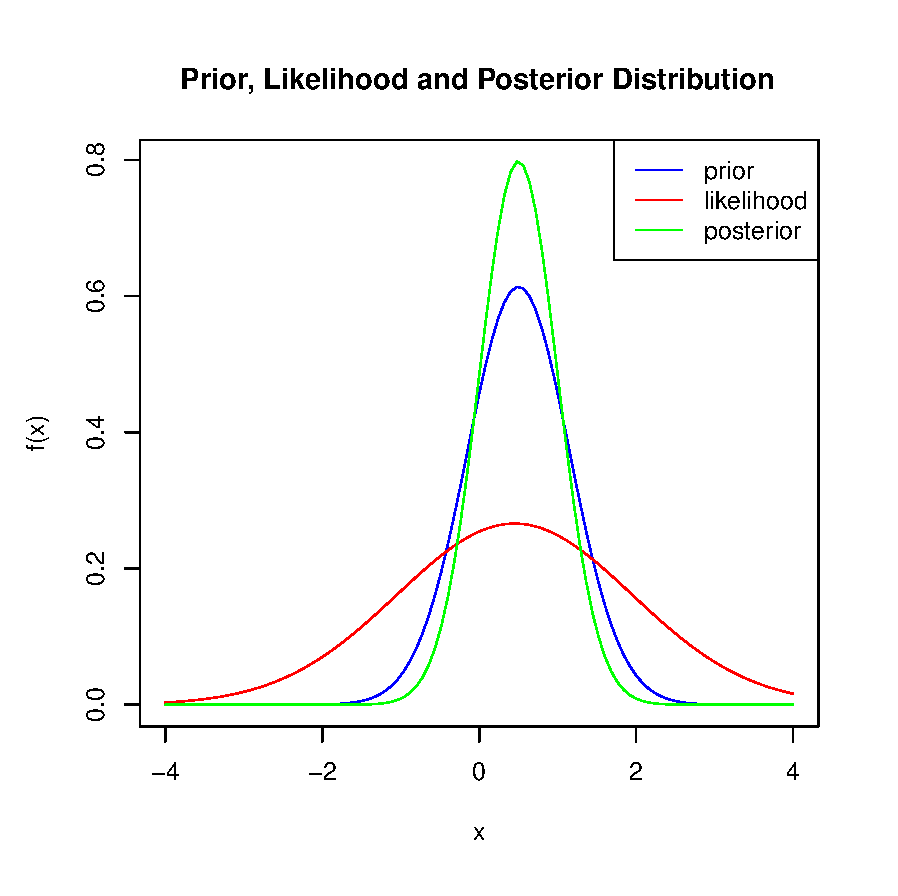
\includegraphics[scale=0.6]{triplot_v1}% Images in 100% size
  \caption{The triplot from first year's data. }
\label{fig:FirstTriplot}
\end{figure} 

\begin{figure}
\centering
 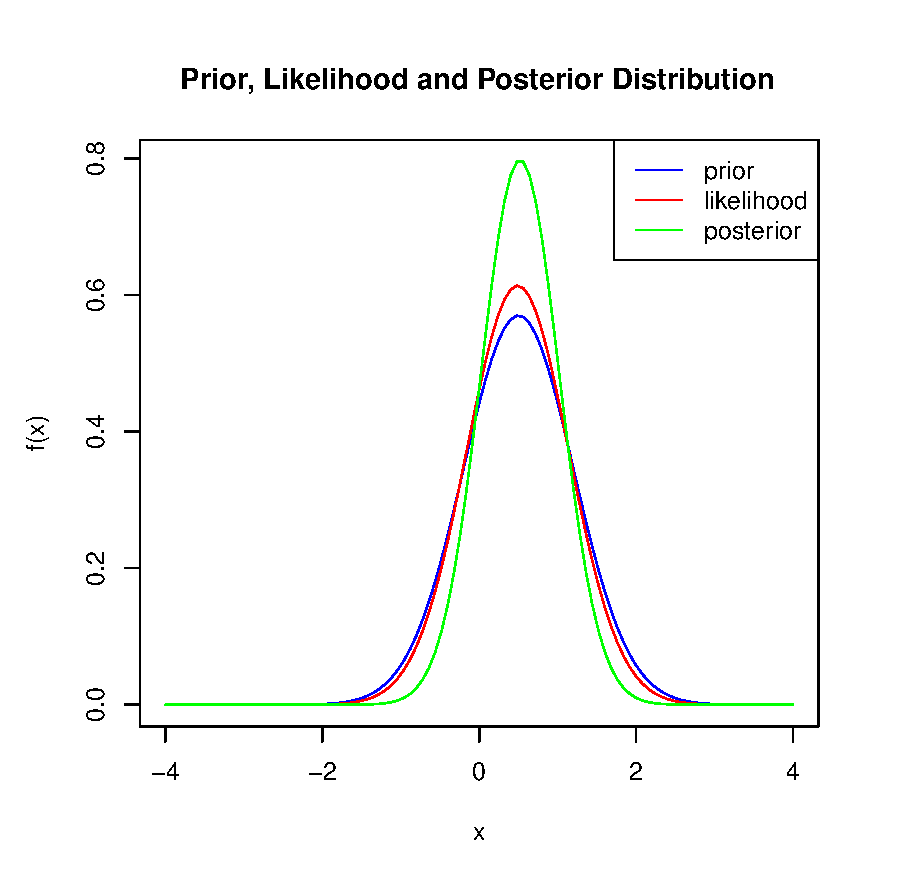
\includegraphics[scale=0.6]{triplot_v2}% Images in 100% size
  \caption{The triplot from two years' data. }
\label{fig:TwoTriplot}
\end{figure} 

\newpage
\section{Sequential Updating}

In the last example we pooled the data from the two years and went back to the original prior distribution to use Bayes' theorem. We did not need to do this. A nice feature of Bayes' theorem is the possibility of updating sequentially, incorporating data as they arrive. In this case, consider the data to be just the new patients observed to a six months follow-up during the second year. These comprise $55$ patients, of whom $28$ had survived. The doctor could consider these as the data $x$ with $n=55$ and $r=28$. What would the prior information be?
\\
Clearly, the prior distribution should express her information prior to obtaining these new data, i.e. after the first years' data, so her prior for this second analysis is her \underline{posterior} distribution form the first. This was $Be(28.28,36.23)$. Combining this prior with the new data gives the same posterior $Be(28.28+28,36.23+27)=Be(56.28,63.23)$ as before. This simply confirms that we can get to the posterior distribution.
\begin{itemize}
\item In a single step, combining all the data with a prior distribution representing information available before any of the data were obtained.
\item Sequentially, combining each item or block of new data with a prior distribution representing information available just before the new data were obtained (but after getting data previously received).
\end{itemize}

\section{Normal Sample}

Let $X_1,X_2,...,X_n$ be from $\mathcal{N}(\mu,\sigma^2)$. $\theta=(\mu,\sigma^2) \rightarrow$ unknown parameters.
The likelihood is:
\begin{equation}
\begin{split}
f(x \mid \mu,\sigma^2)= \prod_{i=1}^{n} \frac{1}{\sqrt{2 \pi} \sigma} \exp \left \{ -\frac{1}{2 \sigma^2}(x_i - \mu)^2  \right \}
\\
\propto \sigma^{-n} \exp \left [  -\frac{1}{2 \sigma^2}  \left \{ n(\bar{x} - \mu)^2 +S^2 \right \} \right ]
\end{split}
\end{equation}
where $S^2=\sum_{i=1}^{n}(x_i - \bar{x})^2$

\section{NIC distributions}

For the prior distribution, we now need a \underline{joint} distribution for $\mu$ and $\sigma^2$

\begin{definition}
The normal-inverse-chi-squared distribution(NIC) has density:
\begin{equation}
f(x \mid \mu,\sigma^2) \propto  \sigma^{-(d+3)^/2}  \exp \left [ -\frac{1}{2 \sigma^2} \left \{ v^{-1}( \mu - m)^2 +a  \right \} \right ]
\end{equation}
where $a>0$, $d>0$ and $v>0$.
\end{definition}
The following facts are easy to derive about $NIC(m,v,a,d)$ distribution. 
\begin{enumerate}
\item The conditional distribution of $\mu$ given $\sigma^2$ is $\mathcal{N}(\mu, v \sigma^2)$ so $E(\mu \mid \sigma^2)=m$, $v(\mu \mid \sigma^2)= v \sigma^2$.
\item The marginal distribution of $\sigma^2$ is such that $a \sigma^{-2} \sim \chi^{2}_d$. We say that $\sigma^2$ has the inverse-chi-square distribution $IC(a,d)$. We have $E(\sigma^2)=a/(d-2)$ if $d>2$ and $v(\sigma^2)=2a^2/\left \{ (d-2)^2 (d-4) \right \}$ if $d>4$.
\item The conditional distribution of $\sigma^2$ given $\mu$ is $IC(v^{-1}(\mu - m)^2+a, d+1)$ and in particular $E(\sigma^2 \mid \mu)= (v^{-1}(\mu - m)^2 +a)/(d-1)$ provided  $d>1$.
\item The marginal distribution of $\mu$ is such that $(\mu - m)\sqrt{d}/\sqrt{ a v}\mu +d$. We say that $\mu$ has $t$-distribution $t_d(m,a v/d)$. We have $E(\mu)=m$ if $d>1$, and $v(\mu)=av/(d-2)$ if $d>2$.
\end{enumerate}
\section{Posterior}
Supposing then that  the prior distribution is $NIC(m,v,a,d)$, we find 
\begin{equation}
f(\mu, \sigma^2 \mid x) \propto \sigma^{d+n+3} \exp \left [ -\frac{1}{2 \sigma^2} \theta \right ]
\end{equation}
where $\theta = v^{-1}(\mu - m)^2 +a +n(\bar{x}-\mu)+s^2$ is a quadratic expression in $\mu$. After completing the square, we see that $\mu, \sigma^2 \mid x \propto NIC(m^*,v^*,a^*,d^*)$ where $m^*=(v^{-1}m + n \bar{x})/(v^{-1}+n)$, $v^*= (v^{-1}+n)^{-1}$, $a^* = a+S^2 +( \bar{x}-m)^2/(n^{-1}+v)$, $d^*=d+n$. To interpret these results, note first that the posterior  mean of $\mu$ is $m^*$ which is a weighted average of the prior mean $m$ and the usual data only-estimate $\bar{x}$ with weights $v^{-1}$ and $n$. 
\\
\\
The posterior mean of $\sigma^2$ is $a^* /(d^* -2)$ which is a weighted average of three terms: the prior mean $a/(d-2)$ with weight $(d-2)$, the usual data-only estimate $S^2/(n-1)$ with weight $(n-1)$ and $(\bar{x}-m)/(n^{-1}+v)$ with weight $1$.
\section{Weak prior}
We clearly obtain \underline{weak prior information about $\mu$} by letting $v$ go to infinity or $v^{-1}\rightarrow0$. Then $m^* = \bar{x}$, $v^* = 1/n$, $a^* = a+S^2$, because the third term disappears.
\\
\\
To obtain weak prior information also about $\sigma^2$, if it is usual to set $a=0$ and $d=1$. Then $a^* = S^2$ and $d^* = n-1$. The  resulting inference match the standard frequentist results very closely with these parameters, since we have:
\begin{equation}
\frac{(\mu - \bar{x})\sqrt{n}}{S/\sqrt{n-1}} \propto t_{n-1},
\end{equation}
\begin{equation}
\frac{S^2}{\sigma^2} \propto \chi^{2}_{n-1}
\end{equation}
Exactly the same distribution statements underlie standard frequentist inference in this problem.

\lecture{Inference}
\underline{\bf{Summarisation:}} Here all inferences are derived form the posterior distribution. In frequentist statistics, there are three kinds of inference:
\begin{itemize}
\item Point estimation: unbiasedness, minimum variance estimation
\item Interval estimation: Credible intervals in Bayesian inference, confidence interval in frequentist approach
\item Hypothesis testing: Signifcance test.
\end{itemize}
In Bayesian inference, the posterior distribution expresses all that is known about $\theta$. So it uses \underline{an appropriate summaries} of the posterior distribution to describe the main features of what we now know about $\theta$.
\\
\\
\underline{\bf{Plots:}} To draw the posterior density 
\begin{figure}
 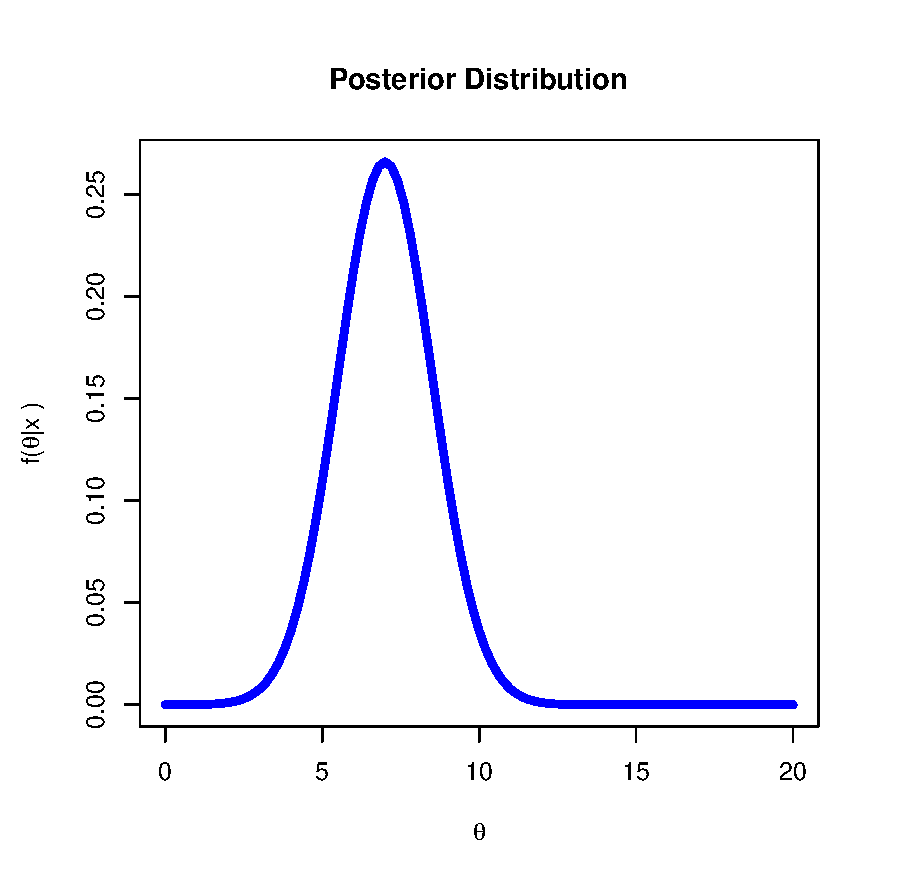
\includegraphics[scale=0.4]{posterior}% Images in 100% size
  \caption{A posterior density plot. }
\label{fig:posterior}
\end{figure} 
\newpage
For a bivariate parameter, we can still usefully draw the density as a perspective plot or a contour plot.

\begin{figure}[h!]
    \centering
    \begin{subfigure}[t]{0.45\textwidth}
        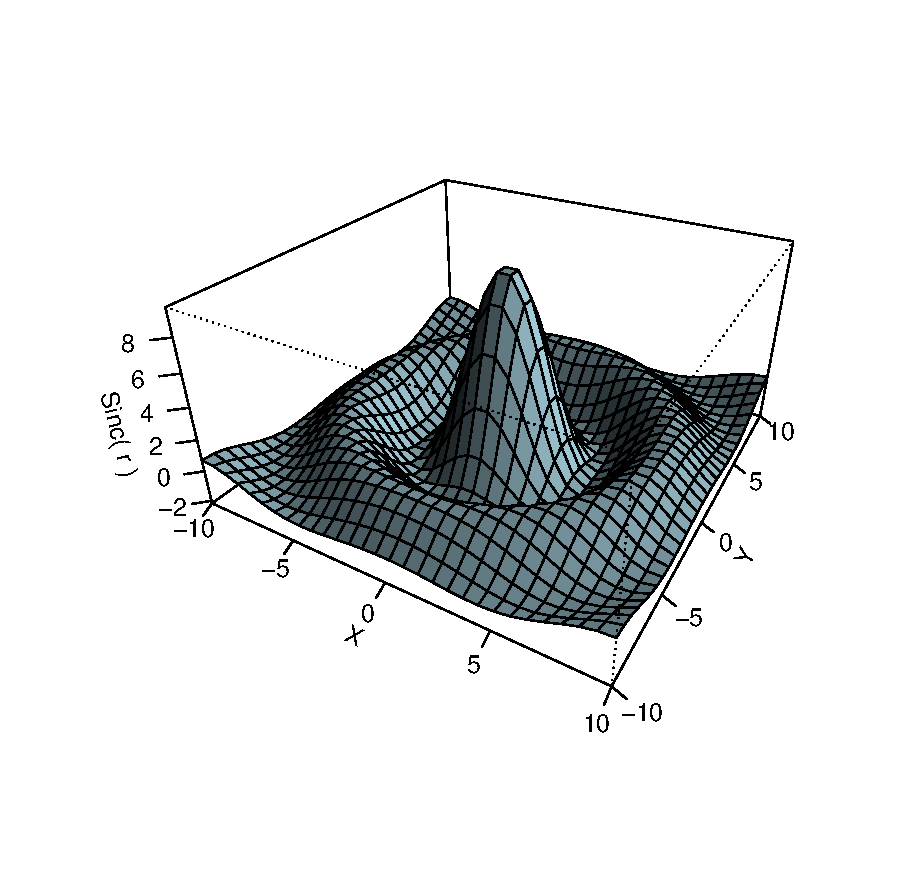
\includegraphics[width=\textwidth]{perspec}
        \caption{Perspective plot}
        \label{fig:perspective}
    \end{subfigure}
\begin{subfigure}[t]{0.45\textwidth}
        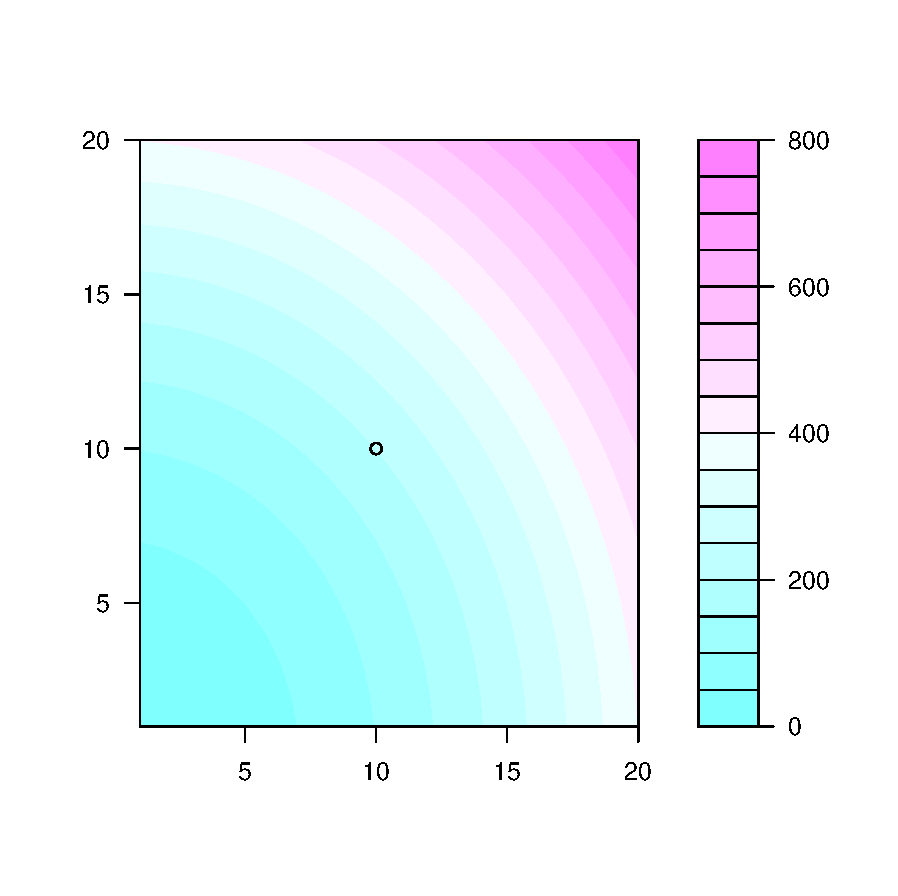
\includegraphics[width=\textwidth]{contour}
        \caption{Contour plot}
        \label{fig:contour}
    \end{subfigure}
\end{figure}

\begin{figure}[h!]
 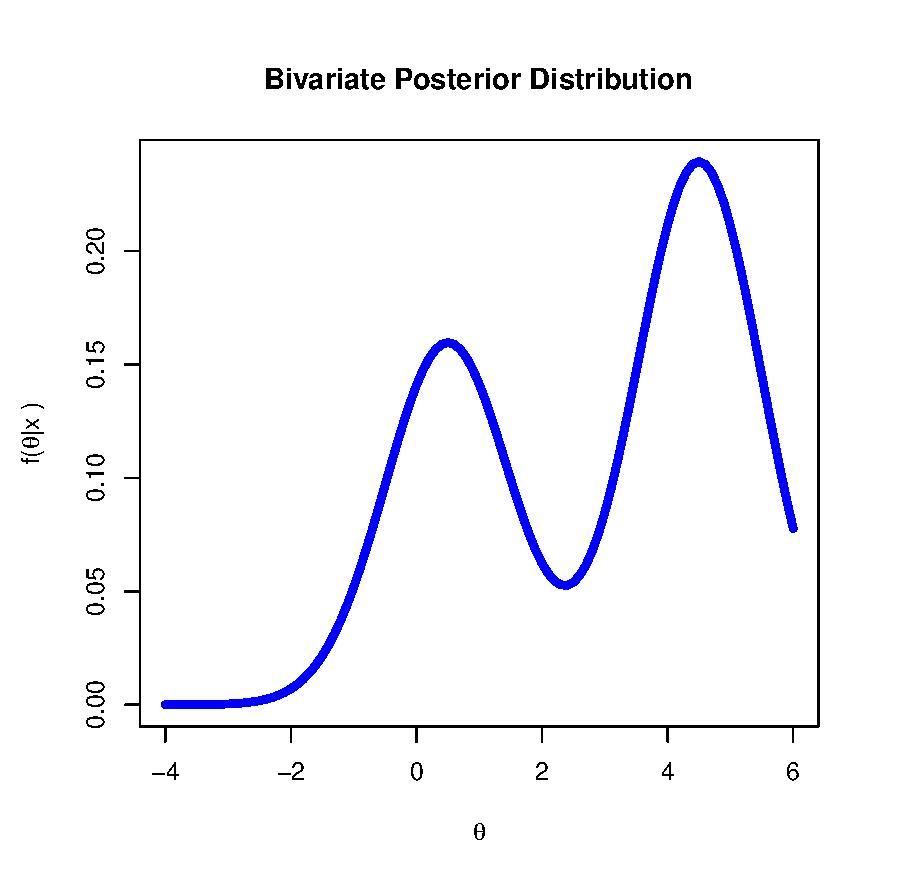
\includegraphics[scale=0.4]{BivarPost}% Images in 100% size
  \caption{Marginal Densities. }
\label{fig:posterior}
\end{figure}
\section{Shape}
In general, plots illustrate the shape of the posterior distribution. Important features of shape are modes (and antimodes), skewness and kurtosis (peakedness or heavy tails). The quantitative summaries of shape are needed to supplement like the view of mode (antimode). 
\\
The first task is to identify turning points of the density, i.e. solutions of $f'(\theta)=0$. Such points include \underline{local maxima} and \underline{minima} of $f(\theta)$ which we call \underline{mode} and \underline{antimode}, respectively.
\\
A point $\theta_0$ is characterized as a mode if $f'(\theta_0)=0$ and $f''(\theta_0)<0$ whereas it is an antimode if $f'(\theta_0)=0$ and $f''(\theta_0)>0$. Any point $\theta_0$ for which $f''(\theta_0)=0$ is a point of inflection of the density (whether or not $f'(\theta_0)=0$).

\begin{example}
Consider the gamma density
\begin{equation}
f(\theta)=\frac{a^b}{\Gamma(b)}\theta^{b-1}e^{-a \theta}\qquad;\qquad \theta>0
\end{equation}
where $a$, $b$ are positive constants.
\begin{equation}
f'(\theta)=\frac{a^b}{\Gamma(b)}\left \{ (b-1) -a \theta  \right \}\theta^{b-2}e^{-a \theta}
\end{equation}

\begin{equation}
f''(\theta)=\frac{a^b}{\Gamma(b)}\left \{a^2 \theta^2 - 2a (b-1)\theta -(b-1)(b-2) \right \}\theta^{b-3}e^{-a \theta}
\end{equation}
So from $f'(\theta)$, the turning point at $\theta=(b-1)/a$. For $b \leq 1$, $f'(\theta)<0$ for all $\theta \geq 0$, so $f(\theta)$ is monotonic decreasing and the mode is at $\theta=0$. For $\theta>1$, $f(\theta) \rightarrow 0$ as $\theta \rightarrow 0$, so the turning point $\theta=0$ is not a mode. In this case, $f'(\theta)>0$ for $\theta < (b-1)/a$ and $f'(\theta)<0$ for  $\theta > (b-1)/a$. Therefore $\theta = (b-1)/a$ is the mode. Looking at $f''(\theta)$, the quadratic expression has roots at $\theta = \frac{b-1}{a}\mp \frac{(b-1)^{1/2}}{a}$. Therefore $b>1$, these are the points of inflection.
\end{example}

\begin{example}
Consider the mixture of two normal distributions
\begin{equation}
f(\theta)=\underbrace{\frac{0.8}{\sqrt{2 \pi}} \exp \left \{-\frac{1}{2} \theta^2 \right \}}_{\sim \mathcal{N} \quad with \quad weight}+ \underbrace{\frac{0.2}{\sqrt{2 \pi}} \exp \left \{-\frac{1}{2} (\theta-4)^2 \right \}}_{\sim \mathcal{N} \quad with \quad weight}
\end{equation}

\begin{figure}[h!]
 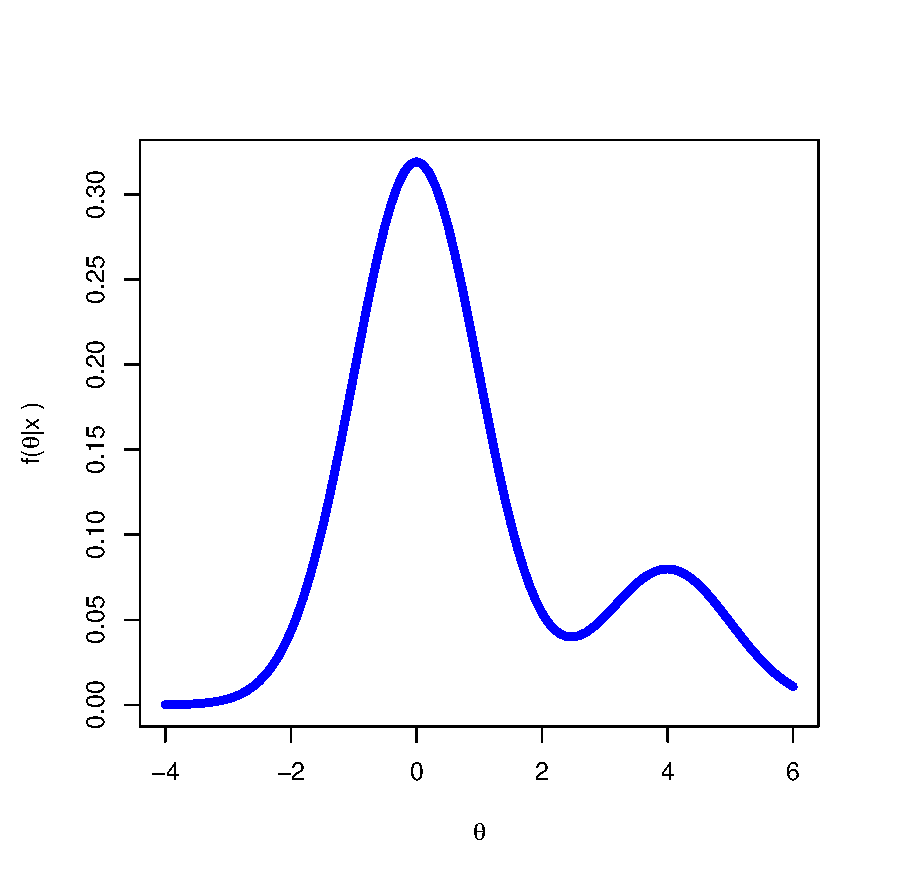
\includegraphics[scale=0.4]{MixGauss}% Images in 100% size
  \caption{Plot of mixture of two normal distributions }
\label{fig:posterior}
\end{figure}

\begin{equation}
f'(\theta)=-\frac{0.8 \theta}{\sqrt{2 \pi}} \exp \left \{-\frac{1}{2} \theta^2 \right \}-\frac{0.2(\theta -4)}{\sqrt{2 \pi}} \exp \left \{-\frac{1}{2} (\theta-4)^2 \right \}
\end{equation}
For $\theta \leq 0$, $f'(\theta)>0$ and for $\theta \geq 0$, $f'(\theta)<0$, the turning points at $\theta=0.00034$, $2.46498$ and $3.9945$.
\begin{equation}
f''(\theta)=-\frac{0.8 (\theta^2-1)}{\sqrt{2 \pi}} \exp \left \{-\frac{1}{2} \theta^2 \right \}-\frac{0.2((\theta^2-8\theta -15)}{\sqrt{2 \pi}} \exp \left \{-\frac{1}{2} (\theta-4)^2 \right \}
\end{equation}
This is positive for $\theta \leq -1$, for $1 \leq \theta \leq 3$ and $\theta \geq 5$, confirming that the middle turning point is an antimode. Calculating $f''(\theta)$ at the other points confirms them to be modes. Finally points of inflection are at $\theta = -0.99998$, $\theta = 0.98254$, $\theta = 3.17903$, $\theta = 4.99971$. 
\end{example}

\section{Visualizing multivariate densities}

\underline{\bf{Turning points:}}
\\
At a mode, or at a turning pons generally, the gradients of function in all directions are zero. Therefore, the turning points are solutions of the simultaneous equations:
\begin{equation}
0= \frac{\partial f(\theta, \phi)}{\partial \phi}= \frac{\partial f(\theta, \phi)}{\partial \theta}.
\end{equation}
The turning points may be classified by examining the symmetric matrix $F''(\theta
, \phi)$ of the second order partial derivatives. For instance, for a bivariate density $f(\theta, \phi)$,
\begin{equation}
F''(\theta, \phi)=\begin{bmatrix}
\frac{\partial^2 f(\theta, \phi)}{\partial \theta^2 } & \frac{\partial^2 f(\theta, \phi)}{\partial \theta \partial \phi }\\ 
\frac{\partial^2 f(\theta, \phi)}{\partial \phi \partial \theta } & \frac{\partial^2 f(\theta, \phi)}{\partial \phi^2 }
\end{bmatrix}
\end{equation}
$F''(\theta, \phi)$ is known as the \underline{Hessian matrix}. The second derivative of $f(\theta)$ ,m a direction $t$ is after differentiating. At a mode, this must be negative in all directions. So that the Hessian matrix is negative definite. Similarly, at an antimode, it is positive definite. In the intermediate case, where $F''(\theta, \phi)$ is indefinite, i.e. has both positive and negative eigenvalues, we have a saddle point. 
\\
If $F''(\theta, \phi)$ is positive definite, regions are:
\\
$F''(\theta, \phi)$ are negative definite, regions are:
\\
$F''(\theta, \phi)$ is indefinite, indefinite curvature.
On the boundaries between these regions, one eigenvalues of $F''(\theta, \phi)$ is zero, so all points on such boundaries are inflection points.
\\
\underline{A point of inflection} corresponds to the second derivative being zero in some direction $t$, therefore inflection points are characterized by $F''(\theta, \phi)$ being singular. In fact, in more than two dimensions, we can further subdivide the regions of indefinite curvature according to how many positive eigenvalues of $F''(\theta, \phi)$ has, and all these subregions are also separated by inflection boundaries.
\\
\underline{\bf{Location:}}
\\
A plot gives a good idea of location, but the conventional location measures for distributions are also useful. These include the \underline{mean, mode and median}.
\\
\underline{\bf{Dispersion:}}
\\
The usual dispersion measure is the variance, or for a multivariate distribution the variance-covariance matrix.
\\
\underline{\bf{Dependence:}}
\\
It is important with multivariate distributions to summarize the dependence between individual parameters. This can be done with correlation coefficients, but plots of regression functions (conditional mean functions) can be more informative.
\section{Informal Inferences}
\begin{enumerate}
\item Point estimation: The obvious posterior \underline{estimate} of $\theta$ is its posterior mean $\hat{\theta}=E(\theta \mid x)$. Modes and medians are also natural point estimates, and they all have intuitively different interpretations. The mean is the \underline{expected value}, the median is the \underline{central value} and the mode is the \underline{most probable} value.
\item Interval estimation: If asked to provide an interval in which $\theta$ probably lies, we can readily derive such a thing from its posterior distribution. For instance, in the density shown on page 1, there is a probability 0.05 to the left of $\theta=3.28$ and also 0.05 to the right of $\theta = 11.84$. So the interval $(3.28,11.84)$ is a $90 \%$ posterior probability for $\theta$. We call such an interval a \underline{credible interval}.
\begin{itemize}
\item If a \underline{frequentist had} found this interval, it means that it would say that if we repeatedly draw samples of data from the same population, and applied the rule that was used to derive this particular interval to each off those datasets, then $90 \%$ of those intervals would contain $\theta$.
\end{itemize}
If a Bayesian approach, there is a posterior probability $0.9$ that $\theta$ lies between $3.28$ between $11.84$.
\begin{definition}
A $100(1-\alpha) \%$ credible set for $\theta$ is a subset $C$ such that:
\begin{equation}
1-\alpha \leq P(C \mid y)= \int_C p(\theta \mid y) \mathrm{d} \theta.
\end{equation}
where integration is replaced by summation for discrete components.
\end{definition}

\begin{definition}
The exact possible coverage of $(1-\alpha)$ can be found by the \underline{highest posterior density} of HPD credible set as the set: 
\begin{equation}
C= \left \{  \theta \in \Theta : p(\theta \mid y) \geq k(\alpha)\right \}.
\end{equation}
where $k(\alpha)$ is the largest constant satisfying $P(C \mid y) \geq 1-\alpha$. 
\end{definition}
For 2-sided credible set, we can generally take the $\alpha / 2$ and $(1- \alpha/2)$ quantiles of $p(\theta \mid y)$ as our $100(1-\alpha) \%$ credible set for $\theta$. This \underline{equal tail} credible set will be equal to the HPD credible set if the posterior is symmetric and unimodal, but will be a bit wider otherwise.

\item Evaluating hypothesis: Suppose we wish to test a hypothesis $H$ which asserts that $\theta$ lies in some region $A$. The Bayesian way to test to the hypothesis is simply to calculate the (posterior) probability that it is true: $P(\theta \in A \mid x)$. 
\end{enumerate}
\section{Multivariate inference}
All the above treated $\theta$ as a scalar parameter. If we have a vector $\mathbf{\theta}$, then in general we can consider inference of the above forms about any scalar function $\phi = g(\theta)$. The inferences are then derived simply from the marginal posterior distribution of $\phi$.

\lecture{Formal Inference}
Suppose that we want to answer a question that falls neatly into the frequentist point estimation framework, "What is the best estimate of $\theta$?". In the frequentist theory, we need to be explicit about what we would regard as good properties for an estimator in order to identify a best one. 
\\
The Bayesian approach also needs to know what makes a good estimate before an answer can be given. This falls into the framework of formal inference. 
\\
Formally, we would seek the estimate that minimises expected square error. So the expectation is derived from the posterior distribution. We want to minimise:
\begin{equation}
\begin{split}
E((\hat{\theta}-\theta)^2 \mid x)= \hat{\theta}^2 - 2 \hat{\theta}E(\theta \mid x)+E(\theta^2 \mid x)
\\
= (\hat{\theta}-E(\theta \mid x))^2 + v(\theta \mid x).
\end{split}
\end{equation}
So the estimate $\hat{\theta}$ that minimises this expected squared error is $\hat{\theta}=E(\theta \mid x)$.
\section{Utility and decisions}
Formal inference aims to obtain \underline{optimal} answer to inference questions. This is done with reference to a measure of how good or bad the various possible inferences would be deemed to be if we knew the true value of $\theta$. This measure is a \underline{utility} function. Formally, $u(d,\theta)$ defines the value of inference $d$ if the true value of the parameter is $\theta$. Formal inference casts an inference problem as a decision problem. A decision problem is characterized by:
\begin{itemize}
\item a set $\Omega$ of possible parameter values
\item a probability distribution for $\theta \in \Omega$
\item a set $D$ of possible decisions
\item utility function $u(d,\theta)$ for $d \in D$ and $\theta \in \Omega$.
\end{itemize}
\underline{The solution is}
\begin{equation}
\boxed{d_{opt}=arg \quad max_d E_{\theta}(u(d, \theta))}
\end{equation}
Here the distribution of $\theta$ is its prior distribution.
\begin{itemize}
\item In inference problems, we generally define a measure of badness of an inference, which we call a loss function $L(d, \theta)$. We can simply define utility to be negative loss, and then the optimal inference is the one which minimises \underline{posterior expected loss}.
\end{itemize}
\subsection{Formal Point Estimation}
The set $D$ is the set of all possible values of $\theta$. We have seen that if we use squared error loss (which is implicitly the measure used by frequentist in considering mean-squared-error of the variance of an unbiased estimator), formally defining $L(\hat{\theta}, \theta)=(\hat{\theta}-\theta)^2$, then the posterior mean is the optimal estimator. If we use absolute error loss $L(\hat{\theta}, \theta)=\left | \hat{\theta}-\theta \right |$, then the optimal estimator is the posterior median.
\subsection{Formal Interval Estimation}
The possible inferences now are interval or, more generally, subsets of possible values of $\theta$. A loss function will penalize an interval if it fails to contain the true value of $\theta$. So the optimal interval is found from this form:
\begin{equation}
\boxed{d_{opt}=\left \{ \theta: f(\theta \mid) \geq t \right \}}
\end{equation}
where $t$ is chosen to obtain the desired $P(\theta \in d_{opt} \mid x)$. Such a credible interval is called a highest (posterior) density interval (HPD interval or HDI).
\begin{example}
From the following figure \ref{fig:credible} which shows $90 \%$ credible interval, it is not HPI.
\begin{figure}[h!]
 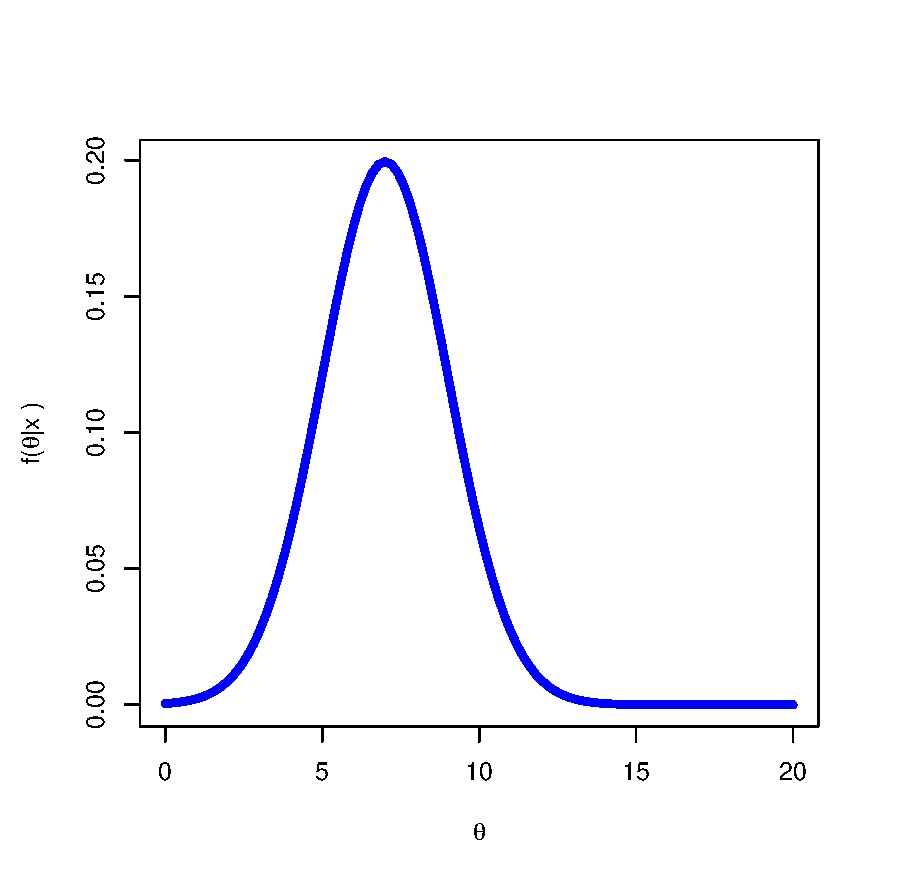
\includegraphics[scale=0.5]{Credible}% Images in 100% size
  \caption{A posterior density plot}
\label{fig:credible}
\end{figure}
Because here the upper and lower limits should have the same posterior density, and shows that the density at $\theta = 3.28$ is higher that at $\theta = 11.84$. So the $90 \%$ highest density interval is actually $(2.78,11.06)$.
\end{example}

\section{Formal Hypothesis Testing}
If we really need to decide whether (to act as if) hypothesis that $\theta \in A$, is true, there are just two inferences. $d_0$ is to say it is true, while $d_1$ says it is false. The loss function will take the form:
\begin{equation}
\begin{split}
L(d_0, \theta)= 0 \quad if\quad \theta \in A
\\
= 1 \quad if \quad \theta \notin A 
\end{split}
\end{equation}
\begin{equation}
\begin{split}
L(d_1, \theta)= k \quad if\quad \theta \in A
\\
= 0 \quad if \quad \theta \notin A 
\end{split}
\end{equation}
where $k$ defines the relative seriousness of the first kind of error relative to the second. Then $E_{\theta}(L(d_0, \theta))=P(\theta \notin A \mid x)$, while  $E_{\theta}(L(d_1, \theta))= k P(\theta \in A \mid x)$. The optimal decision is to select $d_0$ (say that $H$ is true) if its probability $P(\theta \in A \mid x)$ exceeds $\frac{1}{k+1}$. The greater the relative seriousness $k$ of the first kind of error, the more willing we are: 

\section{Nuisance Parameter}
In any inference problem, the parameter(s) that we wish to make inference about is (are) called the \underline{parameter of interest}, and the remainder of components of $\mathbf{\theta}$ is (are) called \underline{nuisance parameters}.
\begin{example}
If we have a sample from $\mathcal{N}(\mu, \sigma^2)$ and we wish to make inference about $\mu$, then nuisance parameter is $\sigma^2$.
\\
If $\mathbf{\theta}=(\phi , \psi)$ and $\psi$ is the vector of nuisance parameters, then the inference about $\phi$ is made from marginal value posterior distribution.
\end{example}
\section{Transformation}
If $\hat{\theta}$ is an estimate of $\theta$, is $g(\hat{\theta})$ the appropriate estimate of $\phi$? 
\\
This depends on the kind of inference being mode. In the particular case of point estimation, then the posterior mean is not invariant in this way.
\begin{example}
If  $\phi = \theta^2)$, then 
\begin{equation}
E(\phi \mid x)=E(\theta^2 \mid x)=v(\theta \mid x)+ E(\theta \mid x)^2 \geq E( \theta \mid x)^2
\end{equation}
The mode is not invariant to transformations but the median is invariant, at least to $1-1$ transformations.
\end{example}
Interval estimates are also invariant to $1-1$ transformations in the sense that if $\left [ a, b \right ]$ is  a $90 \%$ interval, say for $\theta$, then $\left [ g(a), g(b) \right ]$ is a $90 \%$ interval for $\phi$ if g is a monotone increasing function. If $\left [ a, b \right ]$ is a $90 \%$ HPD interval for $\theta$, then $\left [ g(a), g(b) \right ]$ is an HPD interval for $\phi$?


\section{The prior distribution}
The nature of probability:
\begin{enumerate}
\item Frequency probability: Frequentist statistics uses the familiar idea that the probability of an event is the \underline{limiting relative frequency} with which that event would occur in an infinite sequence of repetitions. For this definition of probability to apply, it is necessary for the event to be, at least in principle, repeatable.
\item Personal probability: Bayesian statistics is based on defining the probability of a proposition to be a measure  of a \underline{person's degree of belief} is the truth of that proposition.
\end{enumerate}

In the Bayesian framework, wherever there is uncertainty there is probability.

In particular, parameters have probability distributions.
\section{Subjectivity}

The main critic to Bayesian methods is the subjectivity due to the prior density.

If the data are sufficiently strong, the remaining element of personal judgement will not matter, because all priors based on reasonable interpretation of the prior information will lead to effectively the same posterior inferences. Then we can claim robust conclusion on the basis of the synthesis of prior information and data.

If the data are not that strong, then we do not yet have enough scientific evidence to reach an objective conclusion. Any method which claims to produce a definitive answer in such a situation is misleading, so this is actually a strength of the Bayesian approach.

\section{Noninformative Priors}

The basis of this is that if we have a completely flat prior distribution such that $f(\theta)$ is a constant, then the posterior density if proportional to the likelihood and inferences will be based only on the data. If we can do this, we can get the other benefits of Bayesian analysis, such as having more meaningful inferences that actually answer the question, but without the  supposed disadvantage of subjectivity.

The main problem with this neat solution is that it can not be applied consistently.

\begin{example}
$f(\theta)=1$ for all $\theta \in \left [ 0, 1 \right ]$ uniform distribution represents complete ignorance about $\theta$.

If $\theta$ is ignored, then $\phi = \theta^2$, which also takes values in $\left [ 0, 1 \right ]$, is also completely ignored.

But the implied distribution $f(\phi)=1$ is not consistent with the previous specification of $f(\theta)=1$. The uniform prior distribution for $\theta$ implies that $\phi = \theta^2$ should have the density $f(\phi)=\frac{1}{2 \sqrt{\phi}}$. Conversely, if $\phi$ has a uniform prior distribution, then the implied prior for $\theta$ has density $f(\theta)=2 \theta$.

In general, a uniform prior for $\theta$ translates into a non-uniform prior for any function of $\theta$. Another complication is that if the range of possible values of $\theta$
\end{example}

Another complication is that if the range of possible values of $\theta$ is bounded then we can not properly give it a uniform distribution. For instance, if $\theta \in \left [ 0, \infty \right) $ and we try to define a prior distribution $f(\theta)=c$ for some constant $c$, then there is no value of $c$ that will make this density integrate to $1$. For $c=0$, it integrates to $0$, and for any positive $c$ it integrates to infinity. In these situations, we appeal to proportionality and simply write $f(\theta) \propto 1$

A distribution expressed as $f(\theta) \propto h(\theta)$ when there can not be any proportionality constant that would make this into a proper density function, is called an \underline{improper} distribution. This arises whenever the integral of $h(\theta)$ over the range of possible values of $\theta$ does not change.

\begin{example}
For a parameter $\theta \in \left [ 0, 1 \right ]$, three favourite recommendations are $f(\theta)=1$, $f(\theta)=\pi^{-1} \theta^{-1/2}(1-\theta)^{-1/2}$ and $f(\theta)\propto \theta^{-1} (1-\theta)^{-1}$, the last of these being improper. We can identify these as the $Be(1,1)$, $Be(1/2,1/2)$ and $Be(0,0)$ distributions.
\end{example}

Improper distributions are not in fact usually much of a problem, since we can appeal to proportionality. That is, the absence of a well-defined proportionality constant is ignored and assumed to cancel in the proportionality constant of Bayes' theorem \cite{Gamerman}. In effect, we are obtaining the limit of the posterior distribution as we go through a range of increasingly flat priors towards the uniform limit.

\begin{enumerate}
\item The posterior distribution may also be improper. In this case, technically, the limit of the above process is not well-defined. Improper prior distribution should never be used when the resulting posterior distribution is improper, so it is important to verify propriety of the posterior.
\item When comparing different models for the data, improper distributions always lead to undefined model comparisons. This is an area outside the scope of this course, but very important in practice.
\end{enumerate}

\section{Informative Priors}
So in specifying an informative prior distribution, (a) we specify values for whatever summaries best express the features of the prior information, then (b) we simply choose any conventional $f(\theta)$ that has those summaries.
\begin{example}
I wish to formulate my prior beliefs about number $N$ of students who will turn up to one of my lectures. I first ask myself what my best estimate would be, and I decide on $38$, so I set $E(N)=38$. I next ask myself how far wrong this estimate might be. I decide that the  actual number  could be as high as $48$ or as low as $30$, but I think the probability of the actual number being outside that range is small, maybe only $10 \%$. Now a convenient prior distribution that matches these summaries is the Poisson distribution. 

So it has mean $38$ and $P(30 \leq N \leq 48)=0.87$, which seems a good enough fit to my specified summaries.  
\end{example}

\section{Prior Choices}
There are several alternatives to overcome the problem of improper prior.
\begin{enumerate}
\item \underline{Jeffrey's Prior}:
\\
Let $I(\theta)$ be the Fisher information:
\begin{equation}
I(\theta)=-E \left \{  \frac{\partial^2 \log f(x \mid \theta)}{\partial \theta^2}\right \}.
\end{equation}
In the case of a vector parameter, $I(\theta)$ is the matrix formed as minus the expectation of the matrix of second order partial derivatives of $\log f(x \mid \theta)$. The Jeffrey's prior distribution it then:
\begin{equation}
\boxed{f_o (\theta)\propto \left |  I(\theta) \right |^{1/2}}
\end{equation} 
\begin{example}
If $x_1,x_2,...,x_n$ are normally distributed with mean $\theta$ and known variance $v$, then
\begin{equation}
f(x \mid \theta) \propto \exp \left \{  - \frac{n(\bar{x}-\theta)^2}{2 v}\right \}
\end{equation}
What is the Jeffrey's prior for this distribution?
\\
\textbf{Solution:}\\
\begin{equation}
\log f(x \mid \theta) = - \frac{n(\bar{x}-\theta)^2}{2 v}
\end{equation}

\begin{equation}
\frac{\mathrm{d}^2}{\mathrm{d} \theta^2}\log f(x \mid \theta) = -\frac{n}{2 v}
\end{equation}
Therefore,
\begin{equation}
I(\theta)=-E(\frac{\mathrm{d}^2}{\mathrm{d} \theta^2}\log f(x \mid \theta)) = \frac{n}{2 v}
\end{equation}
As a result,
\begin{equation}
f_0(\theta)= \sqrt{I(\theta)} = \sqrt{\frac{n}{2 v}}.
\end{equation}
\end{example}

\begin{example}
If $x_1,x_2,...,x_n$ are distributed as $\mathcal{N}(\mu,\sigma^2)$ with $\theta=(\mu,\sigma^2)$, then
\begin{equation}
f(x \mid \theta) \propto \sigma^{-n} \exp \left \{  - \frac{-n(s+(\bar{x}-\theta)^2)}{2 \sigma^2}\right \}
\end{equation}
where $s=\frac{\sum (x_i -\bar{x})^2}{n}$, Then what is the Jeffrey's prior of $f(\mu,\sigma^2)$?
\\
\textbf{Solution:}\\
\end{example}

\begin{example}
If $x_1,x_2,...,x_n$ are normally distributed with known mean $m$ and variance $\theta$, then
\begin{equation}
f(x \mid \theta) \propto \theta^{-n/2}\exp \left \{  - \frac{-s}{(2 \theta)^2}\right \}
\end{equation}
where $s=\sum (x_i -m)^2$, then what is the Jeffrey's prior for $\theta$?
\\
\textbf{Solution:}\\
\begin{equation}
\log f(x \mid \theta) =
\end{equation}
\end{example}

A number of objections can made to the Jeffrey's prior, the most important of which is that it depends on the form of the data. The prior distribution should only represent the prior information, and not be influenced by what data are to be collected.
\\

\item \underline{Maximum Entropy}:
\\
The entropy $H(f)=-\int_{-\infty}^{\infty}f(\theta) \log f(\theta) \mathrm{d} \theta$ of the density $f(\theta)$ can be thought of a measure of how uninformative $f(\theta)$ is about $\theta$. For if we try to convert our information about $\theta$ as a general form of inference in the scoring rule framework, $H(f)$ is the lowest obtainable expected loss. If $H(f)$ is high, then the best decision is still poor. Now to represent prior ignorance we could use the prior density $f(\theta)$ which maximizes the entropy.
\begin{example}
Suppose that $\theta$ is discrete with possible values $\theta_1, \theta_2, ..., \theta_k$. The prior distribution with maximum entropy will then maximize $\sum_{i=1}^{k} p_i \log p_i + \lambda \sum p_i$, where $\lambda$ is a Lagrange multiplier, $\partial F / \partial p_i =  \log p_i+1+\lambda$. Equating this to zero yields the solution $p_i=k^{-1}$, $i=1,2,3,...,k$. That is the maximum entropy prior is the uniform distribution. 
\end{example}
The primary criticism of this approach is that it is not invariant under change of parametrization, the problem which the Jeffrey's  prior was designed to avoid. In general, unrestricted maximization of entropy leads to a uniform prior distribution, which was shown to be sensitive to parametrization.
\\
\item \underline{Reference Prior}:
The expected amount of information provided by observing $x$ is given by
\begin{equation}
H\left \{  f(\theta)\right \}-E \left [ H \left \{ f(\theta \mid x) \right \} \right ],
\end{equation}  
where the expectation is over the preposterior distribution of $f(x)$ of $x$. If the experiment yielding $x$ were to be repeated, giving a new observation independent of $x$ given $\theta$ and with the same distribution, the posterior distribution would be expected to show a further reduction in entropy, representing the expected information in the second observation. If this were repeated indefinitely we would eventually learn $\theta$ exactly and so remove all the entropy in the original prior distribution.

In the case of discrete $\theta$ taking a finite of possible values, this process reduces  ??? maximizing prior entropy, and so gives the uniform distribution. This is not the case for continuous $\theta$. It is shown that under appropriate regularity conditions, the reference prior distribution is the Jeffrey prior.
\end{enumerate}

\lecture{Structuring Prior Information}
\underline{Independence}: Suppose that $x_1,x_2,...,x_n$ are a sample from the $\mathcal{N}(\mu ,1)$ distribution, which we write formally as:
\begin{equation}
x_i \mid \mu \sim \mathcal{N}(\mu ,1)
\end{equation}
, independent.  From a  Bayesian perspective, what is meant here is \underline{conditional dependence}. That is the $x_i$'s are independent given $\mu$.

\underline{Exchangaability}: It is same as the independence in frequentist approach.
\begin{definition}
Random variables $x_1,x_2,...,x_m$ are said to be exchangeable if their joint distribution is unaffected by permitting the order of the $x_i$'s.
\end{definition}
So first consider the (marginal) distribution of $x_1$. The definition says that every one of the $x_i$'s must have the same marginal distribution, because we can permute them so that any desired $x_i$ comes into the first position in the sequence. So one implication of exchangeability is that the  random variables in question are identically distributed.

next consider the joint distribution of $x_1$ and $x_2$ Exchangeability means that every pair $(x_i,x_j)$ (for $i \neq j$) has the same bivariate distribution as $(x_1,x_2)$. In particular, the correlation between any pair of random variables is the same.

And so it goes to higher order joint distributions. The joint distributions $(x_1,x_2,....,x_k)$ is the same as that of any other collection of $k$ distinct $x_i$'s. This is the meaning of exchageability.

\begin{itemize}
\item In general, suppose that $x_i$'s have a common distribution $g(x \mid \theta)$, and are independent, given $\theta$. Then the joint density is:
\begin{equation}
\begin{split}
f(x_1,x_2,...,x_m)=\int f(x_1,x_2,...,x_m, \theta) \mathrm{d}\theta
\\
=\int f(x_1,x_2,...,x_m)f(\theta)\mathrm{d}\theta
\\
= \int \prod_{i=1}^{m}g(x_i \mid \theta)f(\theta)\mathrm{d} \theta.
\end{split}
\end{equation}
which is unaffected by permuting the $x_i$'s. Their  common marginal density is:
\begin{equation}
f(x)=\int g(x \mid \theta) f(\theta) \mathrm{d} \theta,
\end{equation} 
and the common distribution of any pair of the $x_i$'s is 
\begin{equation}
f(x,y)=\int g(x \mid \theta)g(y \mid \theta) f(\theta) \mathrm{d} \theta,
\end{equation} 
\end{itemize}

This is generally what a frequentist means by the $x_i$'s being iid, or being a random sample from the distribution $g(x \mid \theta)$. From the Bayesian perspective all frequentist statements are conditional on the parameters. So exchangeability is the Bayesian concept that corresponds very precisely with the frequentist idea of a random sample.

\section{Binary Exchangeability}

\begin{theorem}[De Finetti, 1937]
Let $x_1,x_2,x_3,...$ be an infinite sequence of exchangeable \underline{binary} random variables. Then their joint distribution is characterised by a distribution $f(\theta)$ for a parameter $\theta \in \left [ 0,1 \right ]$ such that the $x_i$'s are independent of $\theta$ with $P(x_i =1 \mid \theta)=0$.
\end{theorem}

De Finetti's theorem says that if we have a sequence of binary variables, so that each $x_i$ takes the value $1$ (success) or $0$ (failure), then we can represent them as independent Bernouilli trials with probability $\theta$ of success in each trial.

\section{Exchangeable Parameters}
Consider the simple one-way analysis of variance model:
\begin{equation}
y_{ij} \sim \left\{\begin{matrix}
\mathcal{N}(\mu_i,\sigma^2), & i=1,2,...,k& \\ 
 &j=1,2,...,n_i &,independent
\end{matrix}\right.
\end{equation}
where $\theta = (\mu_1,\mu_2,...,\mu_k,\sigma^2)$. This says that we have $k$ independent normal samples, where the $i$-th sample has mean $\mu_i$ and size $n_i$, and where all the observations have a common variance $\sigma^2$.

For this model, we need to specify a joint prior distribution for $\mu_1,\mu_2,...,\mu_k$ and $\sigma^2$. Now when it comes to formulating a joint prior distribution for many parameters, it is \underline{much} easier if we can regard them \underline{as independent}. Then we could write:
\begin{equation}
f(\mu_1,\mu_2,...,\mu_k,\sigma^2)=f(\sigma^2) \prod_{i=1}^{k}f(\mu_i),
\end{equation}
and we would only need to specify the prior distribution of each parameter separately. Unfortunately, this is unlikely to be the case in practice with this model.

The model is generally used when the samples are from a related or similar populations. For instance, they might be weight gains of pigs given $k$ different diets, and $\mu_i$ is the mean weight gain with diet $i$. In this sort of situation, the $\mu_i$'s would not be independent. Then we could add to the "prior model"
\begin{equation}
\mu_i \mid \xi, \tau^2 \sim \mathcal{N}(\xi, \tau^2)
\end{equation}
, independent, which says that the $\mu_i$'s are drawn form a normal (assumed) population with unknown mean $\xi$ and unknown variance $\tau^2$.

The prior distribution could then be completed by specifying a joint prior distribution $f(\xi, \sigma^2, \tau^2)$ for the remaining parameters.

\section{Hierarchical Models}

The kind of modelling seen in the previous section is called "hierarchical". In general, we can consider a model of the form:
\begin{itemize}
\item Data model: $f(x \mid \theta)$
\item First level of prior: $f(\theta \mid \phi)$
\item Second level of prior: $f(\phi)$
\end{itemize}
We often refer to $\phi$ as the hyperparameter(s)
\begin{itemize}
\item If we are only interested in the parameter $\theta$ of the original data model,
\begin{equation}
f(\theta)=\int f(\theta \mid \phi) f(\phi) \mathrm{d} \phi.
\end{equation}
\item Let us be actually interested in the hyperparameters $\phi$,
\begin{equation}
f(x \mid \phi)=
\end{equation}
\begin{equation}
f(\theta, \phi)=
\end{equation}
\begin{equation}
f(\theta,\phi \mid x) \propto
\end{equation}
\begin{equation}
f(\theta \mid x)=
\end{equation}
\end{itemize}
\underline{Shrinkage}: It means that the posterior distribution and posterior estimates of these parameters will generally be closer together than their corresponding data estimates. This is a phenomenon known as "shrinkage". Let $w=(\xi, \sigma^2, \tau^2)$ and $\mu=(\mu_1,\mu_2,...,\mu_k)$ and 
\begin{equation}
\begin{split}
f(\mu \mid x, w)\propto f(x \mid \mu, \sigma^2)f(\mu \mid w)
\\
= \prod_{i=1}^{k} \left \{  \prod_{j=1}^{n_i}\frac{1}{\sqrt{2 \pi} \sigma}  \exp \left [  - \frac{(y_{ij}-\mu_i)^2}{2 \sigma^2} \right] \right \}  \exp  \left [- \frac{(\mu_{i}-\xi)^2}{2 \tau^2}\right ]
\\
= \prod_{i=1}^{k}f(\mu_i \mid x, w)
\end{split}
\end{equation}
where each of the $f(\mu_i \mid x, w)$ comes from the analysis of a single normal sample given in Lecture 1. That is conditional on $w$, the $\mu_i$'s are independent $\mathcal{N}(m_{i}^*,v_{i}^*)$, where:
\begin{equation}
v_{i}^* =(n_i \sigma^{-2}+\tau^{-2})^{-1}
\end{equation}
\begin{equation}
m_{i}^* =(n_i \sigma^{-2}+\tau^{-2})^{-1}(n_i \sigma^{-2}\bar{y}_i + \tau^{-2} \xi)
\end{equation}
We can already see the shrinkage in the model, because the posterior mean of each $\mu_i$ is a weighted average of its own data estimate $\bar{y}_i$ and the common value $\xi$. So they are shrunk towards this common value. 
\begin{example}
Let's consider a simple regression situation in which we have observations $y_1,y_2,...,y_n$ at values $x_1<x_2<..<x_n$ of the explanatory variables. The usual linear regression model specifies
\begin{equation}
y_i \mid \alpha, \beta, \sigma^2 \sim \mathcal{N}(\alpha + \beta x_i, \sigma^2)
\end{equation}
Instead we can create the hierarchical model:
\begin{itemize}
\item Data model:
\item First level of prior:
\item Second level of prior:
\end{itemize}
\end{example}
\lecture{Sufficiency and Ancillary}
What happens if $f(x \mid \theta)$ does not depend on $\theta$? If $f(x \mid \theta)$ does not depend on $\theta$, the data are completely uninformative. 
\begin{definition}
$t(x)$ is sufficient if, for any given $\theta$, $f(x \mid \theta)$ is a function only of $t(x)$, apart froma multiplicative factor that can be any function of $x$
\end{definition}

It means that we only need to know $t(x)$ in order to obtain the posterior distribution. It is sufficient to know $t(x)$. Therefore the posterior distribution is the same as if we only had observed $t(x)$ rather than the whole of $x$. 

Suppose that $s(x)$ represents all other information in $x$, $x=(t(x),s(x))$. Then 
\begin{equation}
f(x \mid \theta)=f(t(x) \mid \theta)f(s(x)\mid t(x), \theta).
\end{equation}
$t(x)$ is sufficient $f(s(x)\mid t(x), \theta)$ must not depend on $\theta$. So once we know $t(x)$ there is no information in $s \mid x$.

\begin{definition}
$s(x)$ is ancillary if $f(s(x)\mid \theta)$ does not depend on $\theta$.
\end{definition}

\begin{example}
Let $x_i \mid \sim \mathcal{N}(\mu, \sigma^2)$ with $\sigma^2$ known. Then $x_i-x_j \sim \mathcal{N}(0,2\sigma^2)$ is ancillary for any $i \neq j$. 
\end{example}
\begin{itemize}
\item Let $t(x)$ be the rest of the information in $x$, so that again we have $x=(t(x),s(x))$. Then 
\begin{equation}
f(x \mid \theta)=f(s(x) \mid \theta)f(t(x)\mid s(x), \theta),
\end{equation}
but now this implies that $f(x \mid \theta) \propto f(t(x)\mid s(x), \theta)$
\end{itemize}
\section{The Likelihood Principle}
The likelihood principle asserts that inference should be based only on the likelihood.

\begin{example}
Let $x \sim Be(1, \theta)$ and the results of a fixed number $n$ of independent Bernoullie trials.
\begin{equation}
f_x(x \mid \theta)= \theta^r (1-\theta)^{n-r}
\end{equation}
where $r$ is the number of success. If $x \sim Bi(n,\theta)$, then $f_R (r \mid \theta)= \binom{n}{r}\theta^r (1-\theta)^{n-r} \propto \theta^r (1-\theta)^{n-r}$.

If we keep observing independent Bernoulli trials until we get a fixed number $r$ of success.
\begin{equation}
f_y(y \mid \theta)=\theta^r (1-\theta)^{n-r}
\end{equation}
where $r$-th success on the $n$-th trial. If the distribution is negative binomial 
\begin{equation}
f_N(n)=\binom{n-1}{r-1}\theta^r (1 -\theta)^{n-r} \propto \theta^r (1-\theta)^{n-r}
\end{equation}
\end{example}

\section{Identifiability}
Let $\theta = (y(\theta),h(\theta))$ and $f(x \mid \theta)$ depend only on $g(\theta)$.
\begin{equation}
\begin{split}
f(\theta \mid x) \propto f(x \mid \theta)f(\theta)= f(x \mid g(\theta))f(\theta)
\\
=f(x \mid g(\theta))f(g(\theta))f(h(\theta) \mid g(\theta))
\\
\propto f(g(\theta) \mid x) f(h(\theta) \mid g(\theta)).
\end{split}
\end{equation}
This says that the posterior distribution of $\theta$ is made up of the distribution of $g(\theta)$ and the \underline{prior} distribution of $h(\theta)$ given $g(\theta)$. So it is the \underline{conditional} posterior distribution of $h(\theta)$ given $g(\theta)$ that is the same as the prior. That is 
\begin{equation}
f(h(\theta)\mid x, g(\theta))=f(h(\theta)\mid g(\theta)).
\end{equation}
We say that $h(\theta)$ is \underline{not identifiable} from these data. No matter how much data we get, we can not learn exactly what $h(\theta)$ is. With sufficient data we can learn $g(\theta)$, but not $h(\theta)$.

\section{Asymptotic Theory}

Suppose that we have a sequence of iid observations $x_1,x_2,x_3,...$ and suppose that $\mathbf{x}_n=(x_1,x_2,...,x_n)$ comprises the first $n$ observations. 

We can now consider a sequence of posterior distributions $f(\theta \mid x_1)$, $f(\theta \mid x_2)$, $f(\theta \mid x_3)$,...,$f(\theta \mid x_n)$,$f(\theta \mid x_{n+1})$. We wish to know how the posterior distribution $f(\theta \mid x_n)$ behaves as $n \rightarrow \infty$.

So as we get more data, we expect that the posterior will in some sense converge to the true value. Also, the weight the posterior gives to the data increases, and therefore we can expect that in the limit the posterior will be insensitive to the prior.

Subject to some \underline{regularity conditions}. Regularity conditions:
\begin{enumerate}
\item The whole $\theta$ needs to be identifiable.
\item Prior possibility condition: the prior probability does not give zero probability to the true value of $\theta$.
\item Continuity condition: we need a continuity condition for $\theta$. 
\end{enumerate}
\section{Preposterior Properties}
Let $X$ and $Y$ be any two random variables. Then
\begin{equation}
E(Y)=E\left \{  E(Y \mid X)\right \},
\end{equation}
\begin{equation}
v(Y)=E \left \{  v(Y \mid X)\right \}+ v\left \{  E(Y \mid X)\right \}
\end{equation}
Let's replace $Y$ by the parameter vector $\theta$ and $X$ by the data vector $X$.
\begin{remark}
If we use the posterior mean $E(\theta \mid x)$ to estimate $\theta$, the its expected bias $0$.
\end{remark}

\section{Conjugate Prior Forms}
The conjugacy is a joint property of the prior and the likelihood function that provides a posterior from the same distributional family as the prior.

\begin{example}
Conjugacy in exponential specifications.
\begin{equation}
E(x\mid \theta)=\theta \exp \left \{  -\theta x\right \}
\end{equation}
where $0 \leq x$, $0<\theta$. If $\theta \sim Gamma(\alpha , \beta)$, then
\begin{equation}
f(\theta \mid \alpha, \beta)=\frac{1}{\Gamma(\alpha)}\beta^{\alpha}\theta^{\alpha -1} \exp \left \{  -\beta \theta \right \}
\end{equation}
where $\theta, \alpha, \beta > 0$
\end{example}
Suppose we now observe $x_1,x_2,...,x_n \sim iid$. The likelihood is 
\begin{equation}
L(\theta \mid x)=\prod_{i=1}^{n} \theta e^{-\theta x_i}=\theta^n \exp \left \{  - \theta \sum x_i\right \}
\end{equation}
Thus,
\begin{equation}
\begin{split}
\pi(\theta \mid x) \propto E(x \mid \theta)L(\theta \mid x)
\\
=\theta^n \exp \left \{  - \theta \sum x_i\right \} \frac{1}{\Gamma(\alpha)}\beta^{\alpha}\theta^{\alpha -1} \exp \left \{  -\beta \theta \right \}
\\
\propto \theta^{\alpha +n -1} \exp \left \{  - \theta( \sum x_i + \beta)\right \}
\end{split}
\end{equation}
This is the kernel of a $Gamma(\alpha+n,\sum x_i + \beta)$ and therefore the gamma distribution is shown to be conjugate to the exponential likelihood function.

\begin{table}[h]
\caption{Conjugate Prior Distribution Table}
 \begin{tabular}{||c c c ||} 
 \hline
 Likelihood Form & Conjugate Prior Distribution & Hyperparameters  \\ [0.5ex]
 \hline\hline
 Bernouilli & Beta & $\alpha>0$, $\beta>0$ \\ 
 Binomial & Beta & $\alpha>0$, $\beta>0$   \\ 
 Multinomial & Dirichlet & $\theta_j>0$, $\sum \theta_j=\theta_0$  \\ 
 Negative Binomial & Beta & $\alpha>0$, $\beta>0$  \\ 
 Poisson & Gamma & $\alpha>0$, $\beta>0$  \\
 Exponential & Gamma & $\alpha>0$, $\beta>0$  \\
 Gamma (ind $\chi^2$) & Gamma & $\alpha>0$, $\beta>0$  \\
 Normal for $\mu$ & Normal & $\mu \in \mathbb{R}$, $\sigma^2>0$  \\
  Normal for $\sigma^2$ & Inverse Gamma & $\alpha>0$, $\beta>0$  \\
   Pareto for $\alpha$ & Gamma & $\alpha>0$, $\beta>0$  \\
    Pareto for $\beta$ & Pareto &$\alpha>0$, $\beta>0$  \\
 Uniform & Pareto & $\alpha>0$, $\beta>0$ \\ [1ex] 
 \hline
\end{tabular}
\end{table}

\lecture{Tackling Real Problems}
\appendix

\chapter*{R Codes}

\lstinputlisting[caption={Triplot Code in R}]{BasicStatistics.R}

\lstinputlisting[caption={Inference Plots Code in R}]{Inference.R}


\bibliographystyle{plain}
% Note the spaces between the initials
\bibliography{Bayes}
\end{document}